\section{Method Description}

\subsection{Coverage formula}

Here we proceed with the development of formula for computing the coverage value $c$ an intersecting shape boundary induces on a pixel. The intersecting portion of the border is assumed to be a straight line given by its distance $d$ to the center of the pixel and a phase angle $\phi$ of its normal. The value of $d$ is signed, with negative meaning thath the center is inside the shape.

The pixel is a square with a side of length 1. Therefore, the result $c \in [0, 1]$ is defined as the area of the covered portion. The range of possible $d$ values varies for different~$\phi$, however, the widest range of $[-\frac{\sqrt{2}}{2}, \frac{\sqrt{2}}{2}]$ is achieved for angles $\phi = \frac{2k + 1}{4} \pi$.

First we find the value of $c(\phi, d)$ for $0 \leq \phi \leq \tquarterpi$ and $d \geq 0$. Other arguments are handled using 8-way symmetry:
\begin{gather}
	c(\phi + \frac{2k}{4}\pi, d) = c(\phi, d), \\
    c(\phi + \frac{2k+1}{4}\pi, d) = c(\tquarterpi - \phi, d), \\
    c(\phi, -d) = 1 - c(\phi, d).
\end{gather}

\begin{figure}
	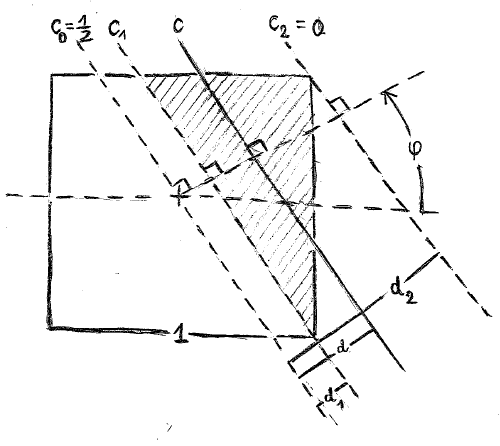
\includegraphics[width=8cm]{img/coverage-formula.png}
    \label{img:coverage-formula}
    \caption{Obtaining coverage induced by line}
\end{figure}

For a given angle Figure \ref{img:coverage-formula} depicts the maximal distance $d_0$ beyond which the pixel stays completely outside. Distance $d_1$ is the point at which the border passes the first corner of the pixel square. The coverage value $c_1 = c(\phi, d_1)$ is equal to the area of the single hatched triangle. Simple geometric inspection gives
\begin{equation}\begin{split}
	d_0 &= \tfrac{\sqrt{2}}{2}\cos(\tquarterpi - \phi), \\
    d_1 &= \tfrac{\sqrt{2}}{2}\cos(\tquarterpi + \phi), \\[3pt]
    c_1 &= \thalf \tan\phi.
\end{split}\end{equation}

When the $d$ falls from $d_0$ to $d_1$, the coverage changes from 0 to $c_1$ quadratically. After that it proceeds linearly to $\thalf$ until $d = 0$. This observation leads to the following formula for the first octant:
\begin{equation}
	c(\phi, d) = \begin{cases}
		\frac{1}{2} - \frac{d}{d_1}\left(\frac{1}{2} - c_1\right)
        	&, 0 \leq d \leq d_1, \\[6pt]
        \left(\frac{d_2 - d}{d_2 - d_1}\right)^2 c_1
        	&, d_1 < d < d_1.
	\end{cases}
\end{equation}